%Pakete;
%A4, Report, 12pt
\documentclass[ngerman,a4paper,12pt]{scrreprt}
\usepackage[a4paper, right=20mm, left=20mm,top=30mm, bottom=30mm, marginparsep=5mm, marginparwidth=5mm, headheight=7mm, headsep=15mm,footskip=15mm]{geometry}

%Papierausrichtungen
\usepackage{pdflscape}
\usepackage{lscape}

%pdf include
\usepackage{pdfpages}

%Deutsche Umlaute, Schriftart, Deutsche Bezeichnungen
\usepackage[utf8]{inputenc}
\usepackage[T1]{fontenc}
\usepackage[ngerman]{babel}

%quellcode
\usepackage{listings}

%tabellen
\usepackage{tabularx}

%listen und aufzählungen
\usepackage{paralist}

%farben
\usepackage[svgnames,table,hyperref]{xcolor}

%font
\usepackage{helvet}
\renewcommand{\familydefault}{\sfdefault}

%Abkürzungsverzeichnisse
\usepackage[printonlyused]{acronym}

%Bilder
\usepackage{graphicx} %Bilder
\usepackage{float}	  %"Floating" Objects, Bilder, Tabellen...

%Kopf- /Fusszeile
\usepackage{fancyhdr}
\usepackage{lastpage}

\pagestyle{fancy}
\fancyhf{} %alle Kopf- und Fußzeilenfelder bereinigen
\fancyhead[L]{Semesterarbeit} %Kopfzeile links
\fancyhead[C]{\project} %Kopfzeile mitte
\fancyhead[R]{Seite \thepage/\pageref{LastPage}} %Kopfzeile rechts
\renewcommand{\headrulewidth}{0.4pt} %obere Trennlinie
\fancyfoot[L]{\jobname} %Fusszeile links
\fancyfoot[C]{Version: \versionnumber} %Fusszeile mitte
\fancyfoot[R]{\today{}} %Fusszeile rechts
\renewcommand{\footrulewidth}{0.4pt} %untere Trennlinie

%Kopf-/ Fusszeile auf chapter page
\fancypagestyle{plain} {
	\fancyhf{} %alle Kopf- und Fußzeilenfelder bereinigen
	\fancyhead[L]{Semesterarbeit} %Kopfzeile links
	\fancyhead[C]{\project} %Kopfzeile mitte
	\fancyhead[R]{Seite \thepage/\pageref{LastPage}} %Kopfzeile rechts
	\renewcommand{\headrulewidth}{0.4pt} %obere Trennlinie
	\fancyfoot[L]{\jobname} %Fusszeile links
	\fancyfoot[C]{Version: \versionnumber} %Fusszeile mitte
	\fancyfoot[R]{\today{}} %Fusszeile rechts
	\renewcommand{\footrulewidth}{0.4pt} %untere Trennlinie
}

\usepackage{changepage}

%links, verlinktes Inhaltsverzeichnis, PDF Inhaltsverzeichnis
\usepackage[bookmarks=true,
bookmarksopen=true,
bookmarksnumbered=true,
breaklinks=true,
colorlinks=true,
linkcolor=black,
anchorcolor=black,
citecolor=black,
filecolor=black,
menucolor=black,
pagecolor=black,
urlcolor=black
]{hyperref} % Paket muss unbedingt als letzes eingebunden werden!

%Dokumenteigenschaften
\providecommand{\project}{WebRTC VoIP Applikation}
\author{Tobias Blaser, Jannis Grimm}
\providecommand{\room}{1.258}
\providecommand{\teacher}{Luc Bläser}
\title{\documentType \project}
\date{\today{}, Rapperswil}


%Dokumenteigenschaften
\providecommand{\documentType}{Domainanalyse}
\providecommand{\versionnumber}{1.0}

\begin{document}

%Titel und Inhaltsverzeichnis
\thispagestyle{empty}
\begin{titlepage}
	\begin{center}

	\vspace*{40mm}
	
	\begin{figure}[htp]
		\centering
		
\includegraphics[scale=0.60]{../img/icon-js-voip.png}
	\end{figure}		
	\vspace*{20mm}
	
	{\fontsize{40}{48} \selectfont \project \\[10mm]}
	{\fontsize{40}{48} \selectfont \documentType \\[5mm]}	
	\vspace*{20mm}
	Tobias Blaser, Jannis Grimm

\end{center}
\end{titlepage}
\clearpage

\chapter*{Änderungsnachweis}
\begin{tabularx}{\textwidth}{|cXlr|} % Versionstabelle, Rahmen links und rechts
		\hline
		\textbf{Version} & \textbf{Änderung} & \textbf{Autor} & \textbf{Datum}\\
		\hline
		1.0 & Dokumentenentwurf & Tobias Blaser & 12.10.2013\\
		1.1 & Architekturanalayse & Tobias Blaser & 12.10.2013\\
		\hline
\end{tabularx}

% Inhaltsverzeichnis
\tableofcontents


\chapter{Einführung}

\section{Beschreibung}
Dieses Dokument beinhaltet die Anforderungen für das Projekt \project.

\section{Gültigkeitsbereich}
Dieses Dokument ist für das gesammte Projekt \project gültig.

\chapter{Domainmodell}

\section{Architekturmodell}
Der logische Aufbau der Software besteht aus vier Schichten:
\begin{figure}[h]
	\centering
	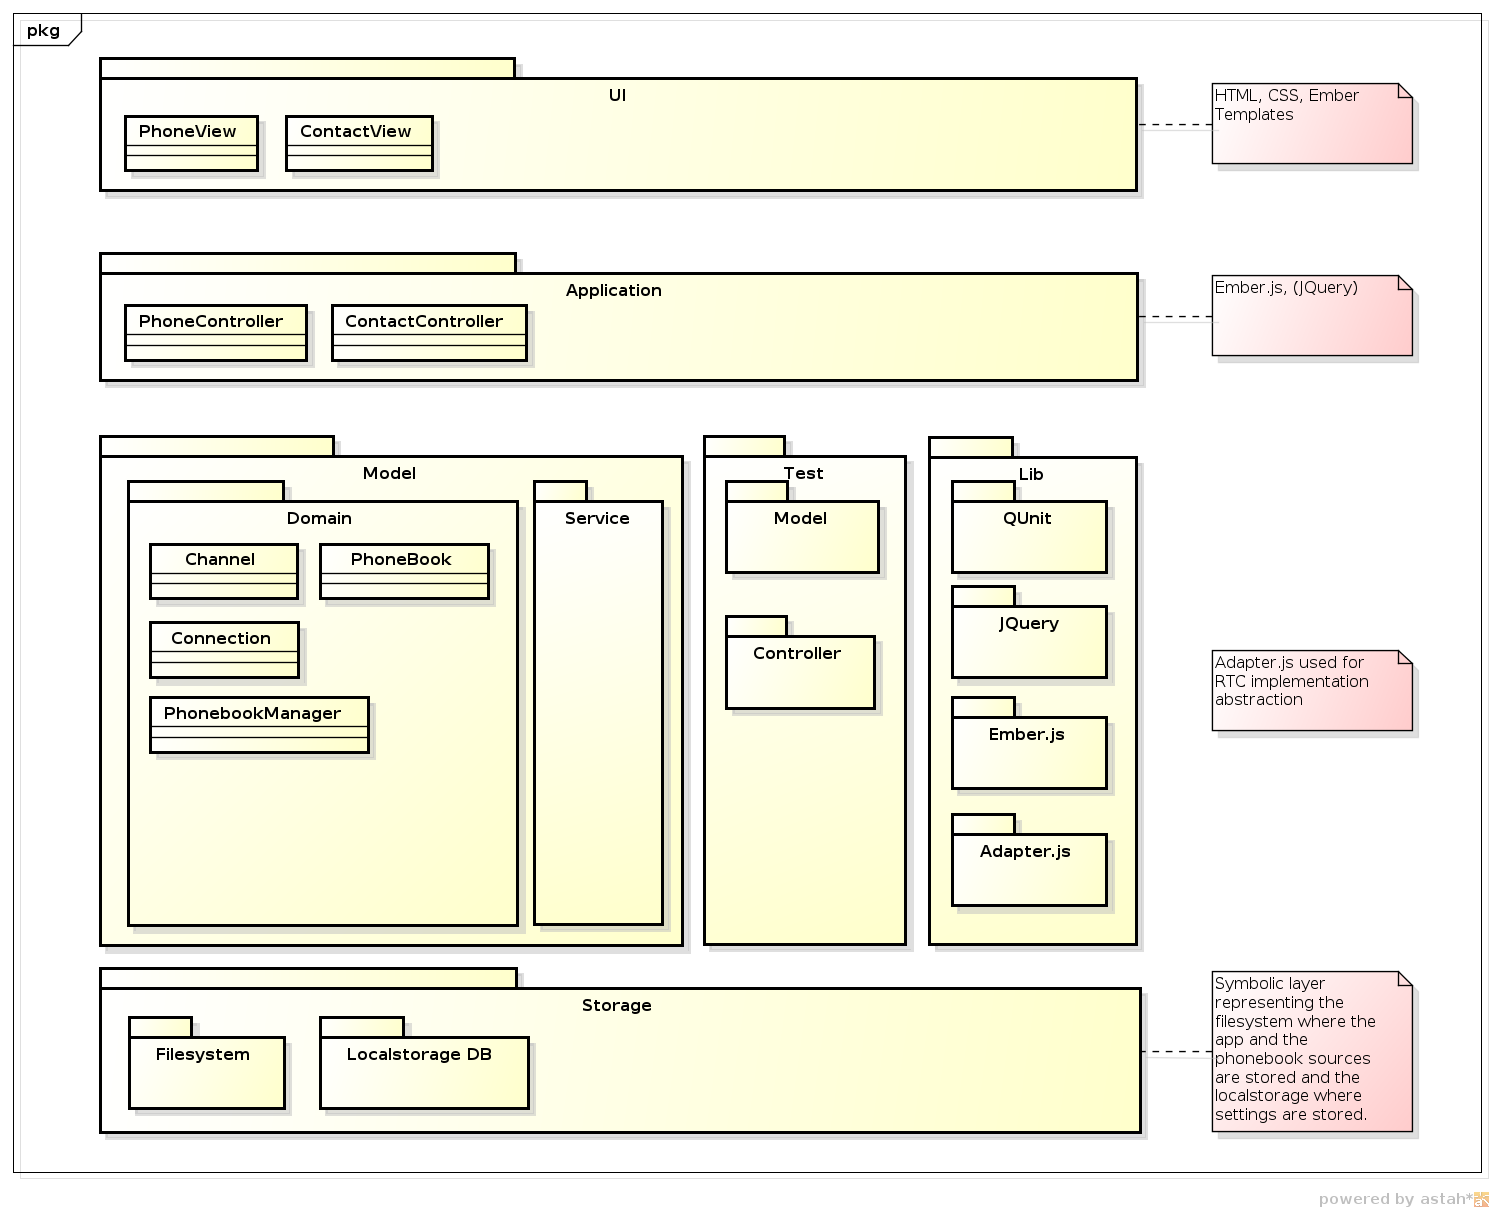
\includegraphics[width=1\textwidth]{img/architecture.png}
	\caption{Architekturdiagramm JS VoIP App}
\end{figure}

\begin{landscape}
\section{Strukturdiagramm}
Im folgenden Diagramm sind die wichtigsten konzeptionellen Klassen und ihre Beziehungen untereinander aufgeführt.
\begin{figure}[h]
	\centering
	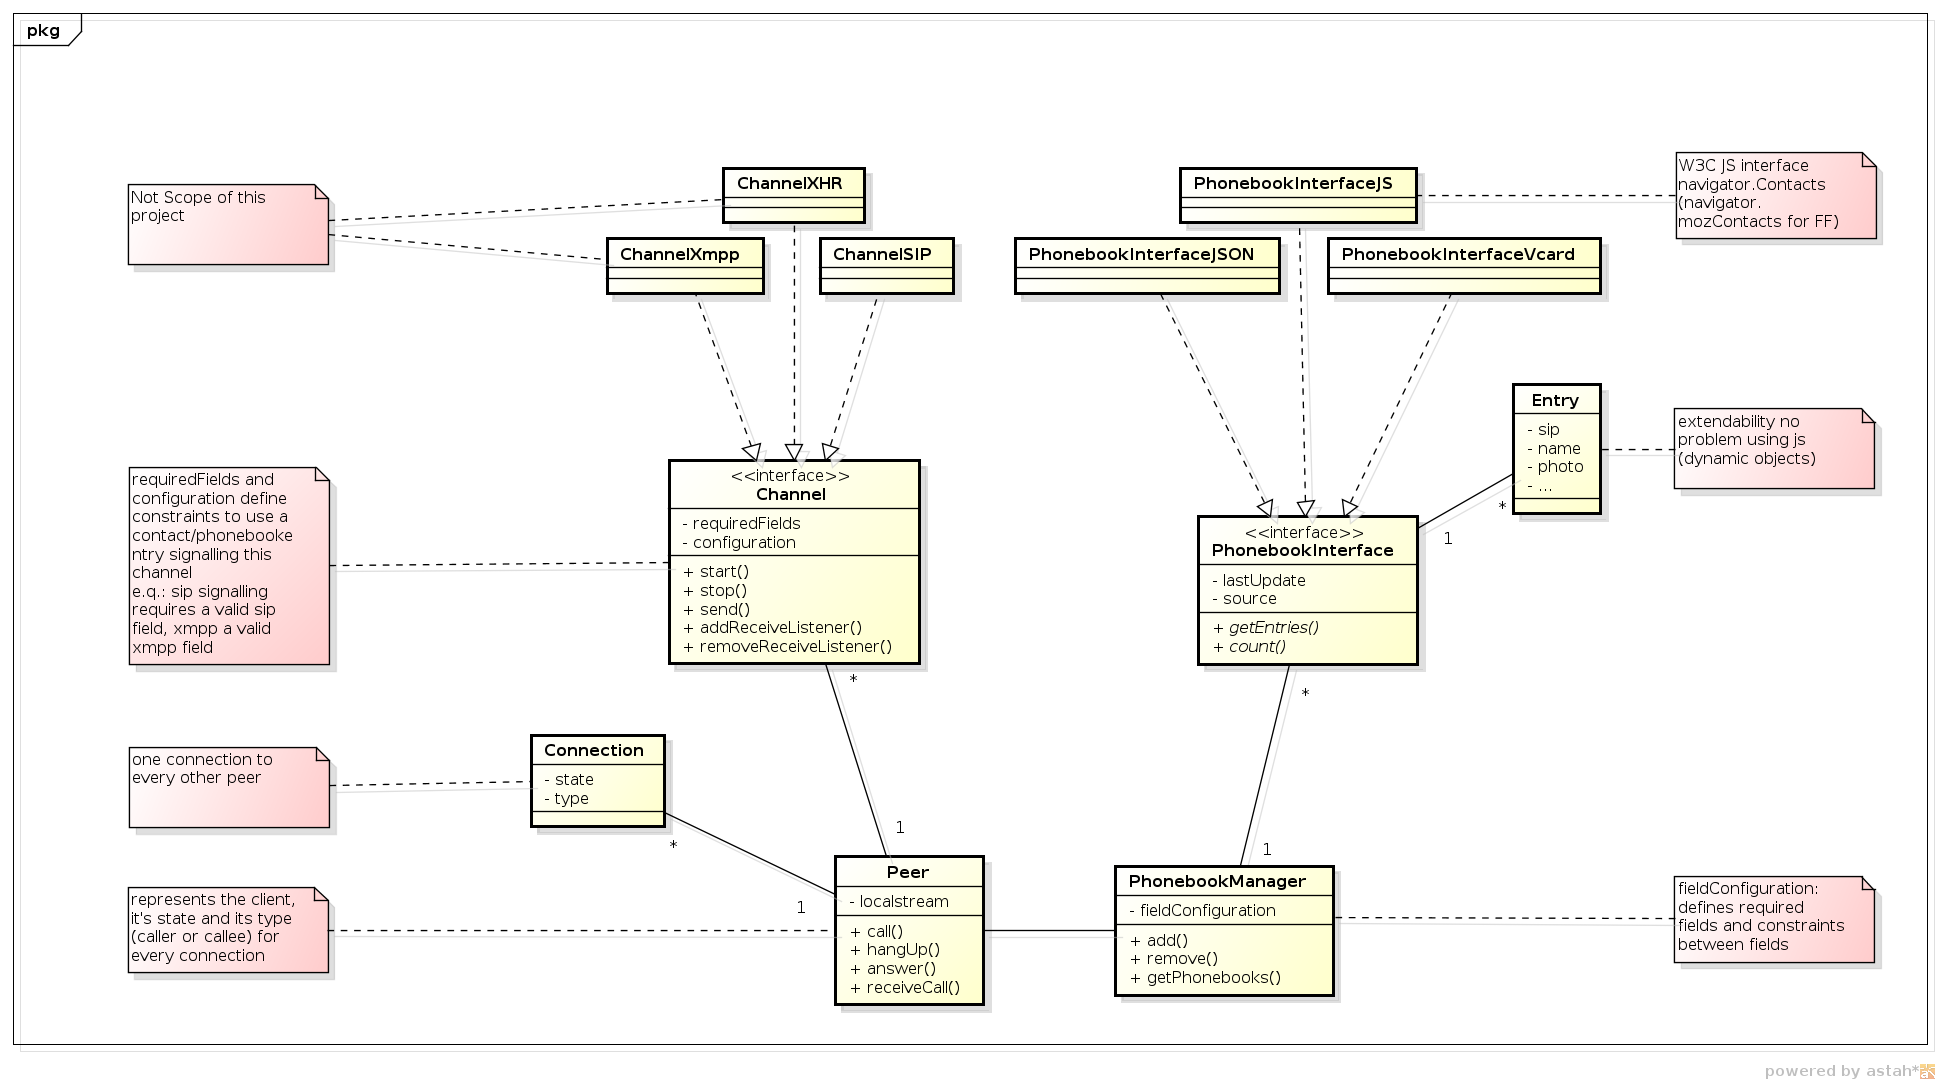
\includegraphics[width=1.2\textwidth]{img/domain.png}
	\caption{Strukturdiagramm JS VoIP App}
\end{figure}
\end{landscape}
\clearpage

\section{Deployment}
Die Applikation wird als ZIP-Datei ausgeliefert oder auf einem Webserver zur Verfügung gestellt. Der Benutzer kann die Datei entpacken und die darin enthaltene HTML Datei mit seinem Browser öffnen.
\begin{figure}[h]
	\centering
	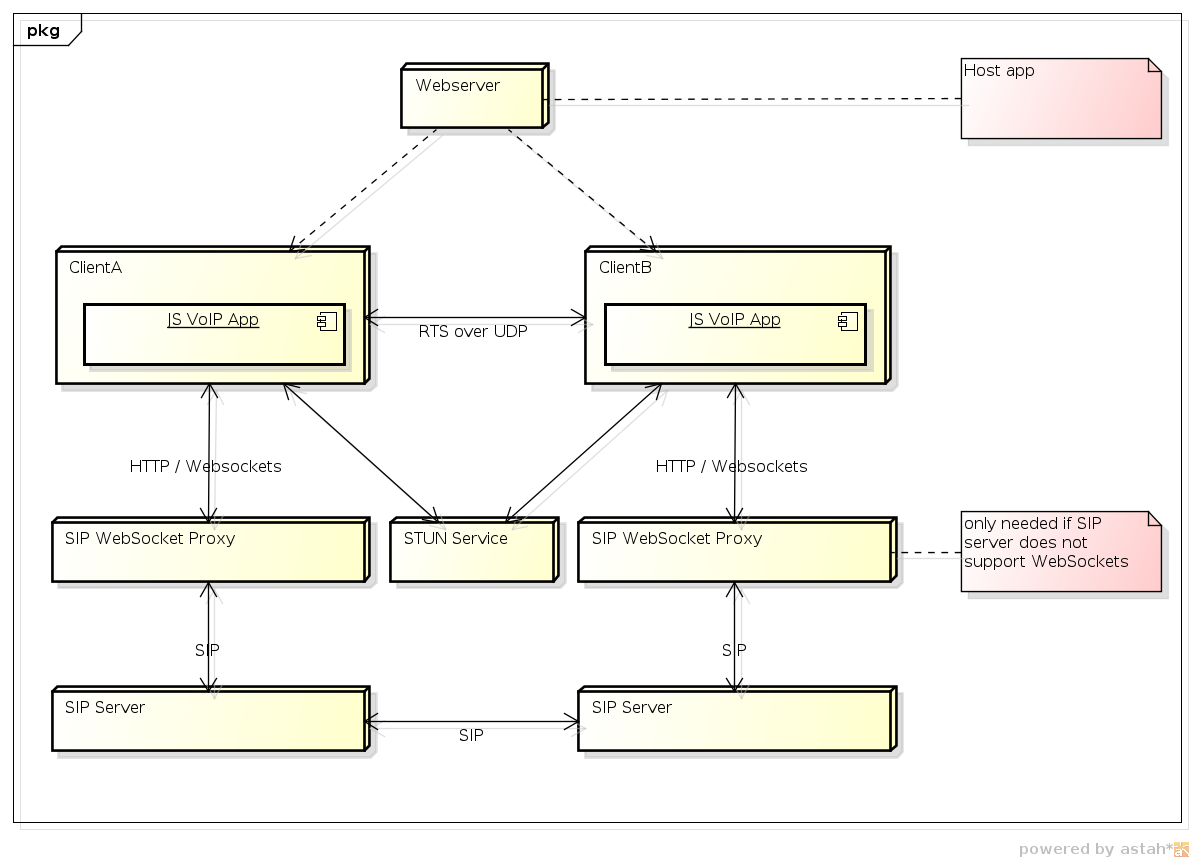
\includegraphics[width=1\textwidth]{img/deployment.png}
	\label{img:deployment}
	\caption{Deploymentdiagramm JS VoIP App}
\end{figure}



\end{document}
